%%%%%%%%%%%%%%%%%% USAGE INSTRUCTIONS %%%%%%%%%%%%%%%%%%
% - Compile using LuaLaTeX and biber, unless there is a particular reason not to. Do not use the older LaTex/PDFLaTeX or BibTeX. (The fonts won't work correctly.)
% - Font and the report 'year' must be specified when all \documentclass or the template won't work correctly. (There's no error checking/default cases!)
% - For best performance save images/graphics as PDF files, not as png/jpg/eps. This makes no difference to how images are inserted using \includegraphics.
% - As many further packages as wanted can be loaded. Below are just an example set. Note that template itself loads a number of packages, including hyperref.
% - References are handed using biblatex.
% - Link to the presentation of theses policy: https://documents.manchester.ac.uk/DocuInfo.aspx?DocID=2863

%%%%%%%%%%%%%%%%%% META DATA SETUP %%%%%%%%%%%%%%%%%%
% This is where the document title and author are set. Other details for the title page are set later
% Note that if/when you edit these you may need to 'Recompile from scratch' to get the changes to display in the PDF. (In Overleaf, select the down arrow to the right of the 'Recompile' button)
\begin{filecontents*}{\jobname.xmpdata}
    \Title{Vision Based Trajectory Tracking of a Low Cost Two Wheel Self Balancing Robot Platform} % title of your thesis
    \Author{Winston Scott 107067151} % should be student number rather than name to help with annoymous marking
    \Language{en-GB}
    \Copyrighted{True}
    % More meta-data fielda can be added here if wanted, see https://ctan.org/pkg/pdfx?lang=en for fields
  \end{filecontents*}
  %%%%%%%%%%%%%%%%%% DOCUMENT SETUP %%%%%%%%%%%%%%%%%%
  \documentclass{uom_eee_dissertation_casson} 
  %%%%%%%%%%%%%%%%%% PACKAGES AND COMMANDS %%%%%%%%%%%%%%%%%%
  % Packages
  \usepackage{graphicx,psfrag,color} % for postscript graphics files
    \graphicspath{ {../../Charts/} }
  \usepackage{amsmath}               % assumes amsmath package installed
    \allowdisplaybreaks[1]           % allow eqnarrays to break across pages
  \usepackage{amssymb}               % assumes amsmath package installed 
  \usepackage{url}                   % format hyperlinks correctly
  \usepackage{rotating}              % allow portrait figures and tables
  \usepackage{multirow}              % allows merging of rows in tables
  \usepackage{lscape}                % allows pages to be typeset in landscape mode
  \usepackage{tabularx}              % allows fixed width tables
  \usepackage{verbatim}              % enhanced version of built-in verbatim environment
  \usepackage{footnote}              % allows more control over footnote environments
  \usepackage{float}                 % allows H option on floats to force here placement
  \usepackage{booktabs}              % improve table line spacing
  \usepackage{lipsum}                % for adding dummy text here
  \usepackage[base]{babel}           % for proper hypthenation in lipsum sections
  \usepackage{subcaption}            % for multiple sub-figures in a single float
  % Add your packages here
  
  % Optional: for adding alt-text to images:
  %\usepackage{pdfcomment}            % for alt text for accessibility
  % Then to add images use:
  % \pdftooltip{\includegraphics[width=0.5\textwidth]{image.pdf}}{Alt-text here}
  % This makes the text in the image non-select-able though (assuming it's a vector file)
  
  % Custom commands
  \newcommand{\degree}{\ensuremath{^\circ}}
  \newcommand{\sus}[1]{$^{\mbox{\scriptsize #1}}$} % superscript in text (e.g. 1st)
  \newcommand{\sub}[1]{$_{\mbox{\scriptsize #1}}$} % subscript in text
  \newcommand{\sect}[1]{Section~\ref{#1}}
  \newcommand{\fig}[1]{Fig.~\ref{#1}}
  \newcommand{\tab}[1]{Table~\ref{#1}}
  \newcommand{\equ}[1]{(\ref{#1})}
  \newcommand{\appx}[1]{Appendix~\ref{#1}}
  %%%%%%%%%%%%%%%%%% REFERENCES SETUP %%%%%%%%%%%%%%%%%%
  % Setup your references here. Change the reference style here if wanted
  \usepackage[style=ieee,backend=biber,backref=true,hyperref=auto]{biblatex}
  % Note backref=true adds a page number (and hyperlink) to each reference so you can easily go back from the references to the main document. You may prefer backref=false if you need to stick strictly to a given reference style
  % Fixes which can't be applied in the .cls file
  \DefineBibliographyStrings{english}{backrefpage = {cited on p\adddot},  backrefpages = {cited on pp\adddot}}
  %  \renewcommand*{\bibfont}{\large}
  % Add more .bib files here if wanted
  \addbibresource{references.bib}
  
  %%%%%%%%%%%%%%%%%% START DOCUMENT %%%%%%%%%%%%%%%%%%
  % Don't edit these lines, title and author are automatically taken from the document meta-data defined above
  \begin{document}
  \makeatletter
  \title{\xmp@Title}
  \studentid{\xmp@Author}
  \makeatother
  
  % Set the below yourself
  \course{Mechatronics and Robotics Engineering}  % "Master of Science in" is added automatically
                                                     % Our courses are: Advanced Control and Systems Engineering, Advanced Control and Systems Engineering with Extended Research, Communications and Signal Processing, Communications and Signal Processing with Extended Research, Electrical Power Systems Engineering, Advanced Electrical Power Systems Engineering, Renewable Energy and Clean Technology, Renewable Energy and Clean Technology with Extended Research
  \submitdate{2024}                                  % regulations ask only for the year, not month
  \wordcount{1000}		                            % use \wordcount{} to set the count, \thewordcount to print in the text
  \maketitle

  %%%%%%%%%%%%%%%%%% LISTS OF CONTENT %%%%%%%%%%%%%%%%%%
  \uomtoc
  % other lists are not required, but can include \uomlof and \uomlot if really want to

  %%%%%%%%%%%%%%%%%% ABSTRACT %%%%%%%%%%%%%%%%%%
  \begin{abstract} % put abstract here. Limit is 1 page.
    This is abstract text.
  \end{abstract}%
  \clearpage
  %%%%%%%%%%%%%%%%%% SECTION 1 %%%%%%%%%%%%%%%%%%
  \section{Introduction}
    \subsection{Background and motivation}
    \subsection{Aims and objectives}
    \subsection{Report structure}
  %%%%%%%%%%%%%%%%%% SECTION 2 %%%%%%%%%%%%%%%%%%
  \section{Literature review} % edit section heading as appropriate
    \subsection{Introduction}
      \subsection{Summary}
  %%%%%%%%%%%%%%%%%% SECTION 3 %%%%%%%%%%%%%%%%%%
  \section{Methodology } % edit section heading as appropriate
    \subsection{System Design and Modeling }
    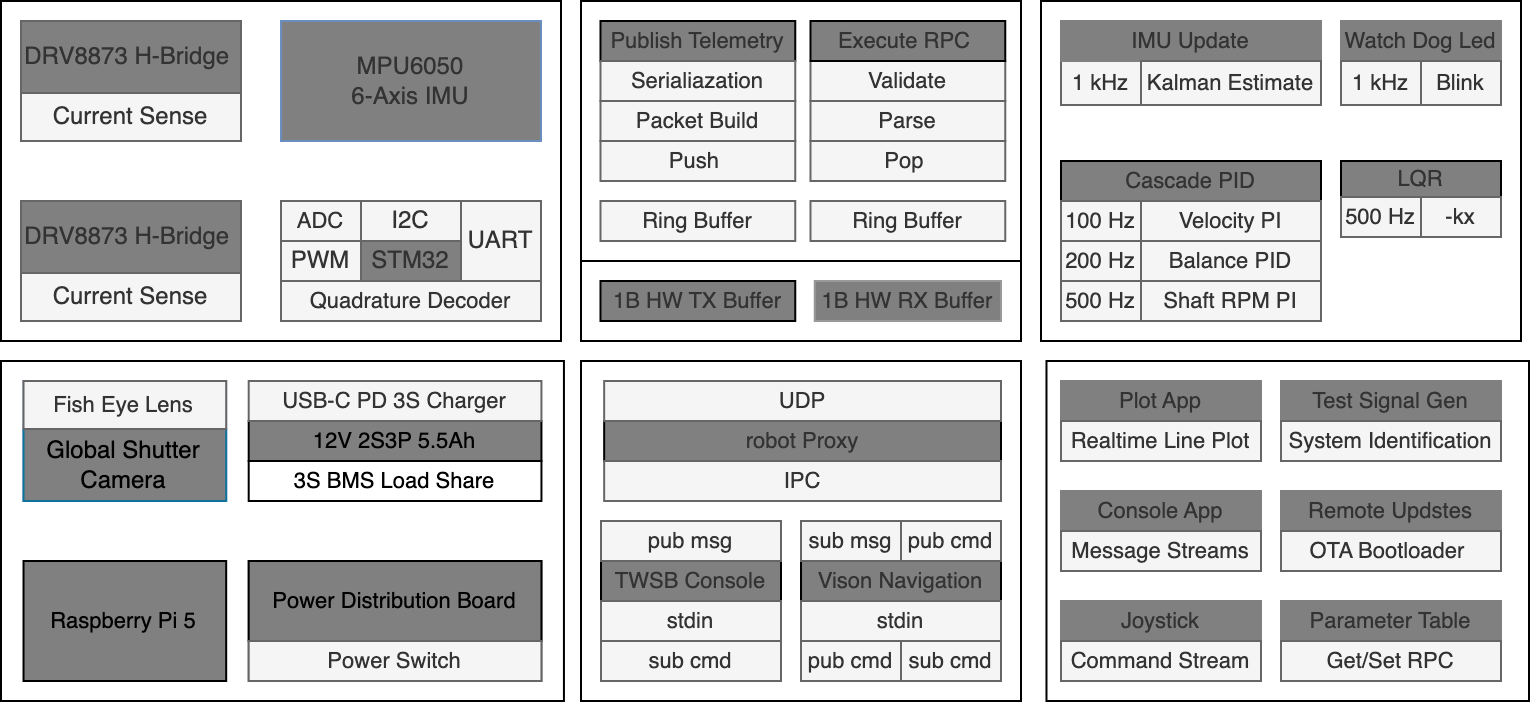
\includegraphics[width=\textwidth]{SystemOverview.png}

    
    \subsection{State Space Model}
        \subsection{2D Kinematics}
        \subsection{3D Dynamics}
        \subsection{DC Motor Model}
        \subsection(Parameter Estimation)
    \subsection{Software Architecture}
        \subsection{Compute Systems Overview }
    \subsection{State Estimation}
        \subsection{Sensor Overview}
        \subsection{Kalman Filter}
        \subsection{Extended Kalman Filter}
        \subsection{DataDriven Techniques}
        \subsection{Adaptive Filter Estimation}
        \subsection{Curvilinear Transformation}
            The planar two wheel self balancing robot, now moddled as a point P, subject to the differential drive constraints, 
            can be instantaneously described as follwing some segment or radius r. This arc seggment forms part of a coninuous spline. 
            The curvature of the spline is given by the inverse of the radius of the circle that best fits the arc segment.
            Where a positive curvature indicates a right turn and a negative curvature indicates a left turn.
            The forward direction is x, and left if y. using the side of the angle between the robtos heading and the observed center line can be used as the derivative term.
            adding the curvature K, 
        \subsection{Vision System}
            \subsection{Pipeline}
            \subsection{Camera Calibration}
            \subsection{IMU Based Software Stabilization}
            \subsection{Adaptive Filters}
            \subsection{Perspective Transformation}
            \subsection{Polynomial Fitting}
        \subsection{Trajectory Generation}
        \subsection{Control System}
            \subsection{Cascade PID}
            \subsection{LQR}
            \subsection{Trajectory Tracking}

  %%%%%%%%%%%%%%%%%% SECTION 4 %%%%%%%%%%%%%%%%%%
  \section{Results and discussion} % edit section heading as appropriate
    \subsection{Introduction}
      \subsection{Detail}
      \subsection{More detail}
      \subsection{Summary}
  %%%%%%%%%%%%%%%%%% SECTION 5 %%%%%%%%%%%%%%%%%%
  \section{Conclusions and future work} % edit section heading as appropriate
    \subsection{Conclusions}
      \subsection{Future work}
  %%%%%%%%%%%%%%%%%% REFERENCES %%%%%%%%%%%%%%%%%%
  %\clearpage % uncomment to start on a new page if wanted
  \printbibliography[title={References},heading=bibintoc] % a single list of references for the whole thesis
  %%%%%%%%%%%%%%%%%% APPENDICES %%%%%%%%%%%%%%%%%%
  \begin{uomappendix} 
      \section{Code}
      \section{Risk assessment}
      Risk assessment is a required appendix. Put here.
      %\section{Other appendices as necessary}
  \end{uomappendix}
  
  %%%%%%%%%%%%%%%%%% END MATTER %%%%%%%%%%%%%%%%%%
  \end{document}